\documentclass{standalone}
\usepackage{tikz,ifthen}
\usepackage{xcolor}
\begin{document}
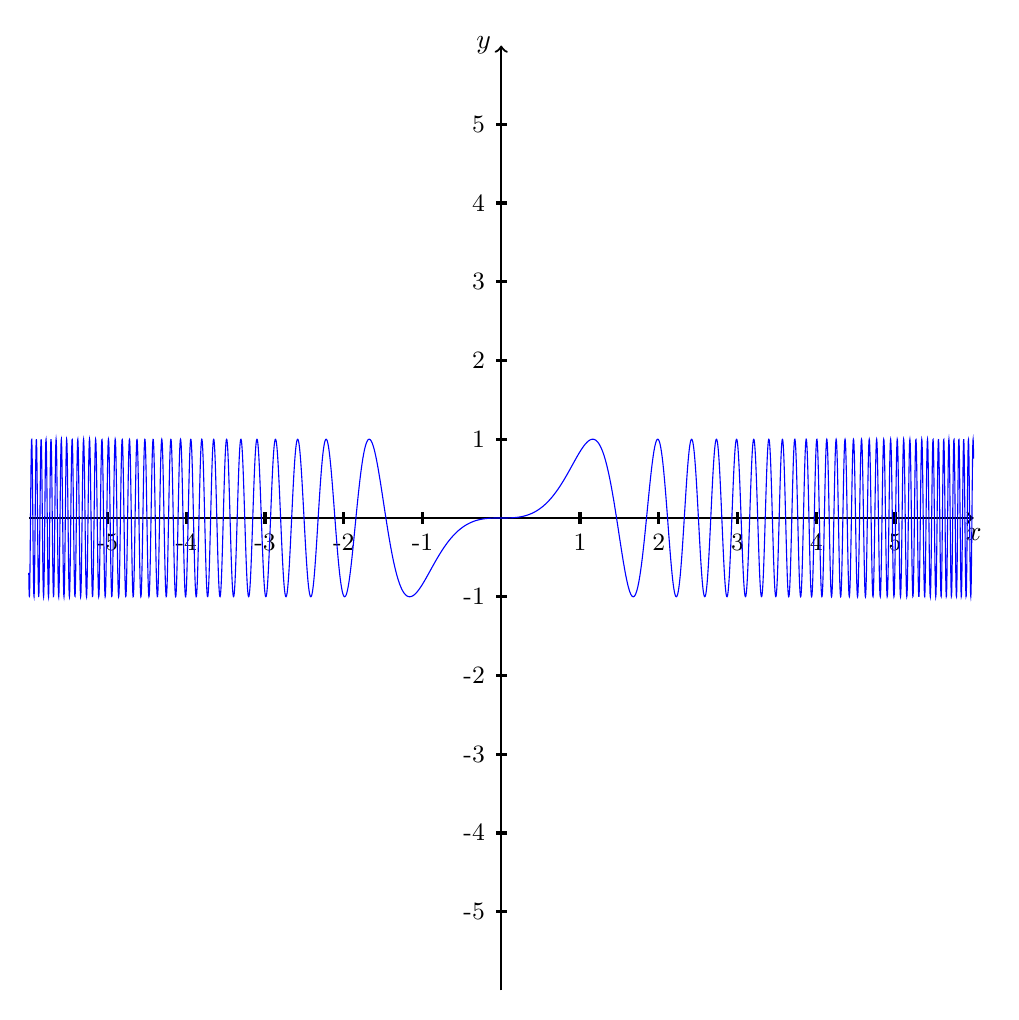
\begin{tikzpicture}
    \draw [thick, ->] (-6,0)--(6,0) node [below] {$x$};
    \draw [thick, ->] (0,-6)--(0,6) node [left] {$y$};
    \foreach \x in { -5, ...,5 }{
        \ifthenelse{\NOT \x = 0}{
            \draw [very thick] (\x,2pt)--(\x,-2pt) node [below, black ] {\small\x};
            \draw [very thick] (2pt,\x)--(-2pt,\x) node [left, black ] {\small\x};
        }{}
    }
    \draw[color=blue,domain=-6:+6,smooth,samples=5724]   plot (\x,{sin(\x*\x*\x r)});

\end{tikzpicture}
\end{document}
